\documentclass[../main.tex]{subfiles} % Due to use of package subfiles

%%%%%%%%%%%%%%%%%%%%%%%%%%%%%%%%%%%%%%%%%%%%%%%%%%%%%%%%%%%%%%%%%%%%%%%%%%%%%%%%

\begin{document}

% \chapter{Lattice Schwinger Model and Confinement} \label{chap:Confinement}
\chapter{Confinement in the Lattice Schwinger Model} \label{chap:Confinement}


In this chapter one of the uses of the (1+1)-dimensional lattice Schwinger model is examined, namely the use of the Schwinger model as a ''toy model'' for quantum chromodynamics. More specifically we will be examining the properties of confinement and string breaking. In \cref{sec:Confinement} the two above mentioned phenomenons are described, and in \cref{sec:LatticeSchwingerModelAndConfienemt} the properties are examined analytically and numerically (\cref{sec:ConfienementAndStringBreakingAnalyticalAndNumerical}) after the lattice Schwinger model Hamiltonian is converted to fit the requirements of a spin-1 gauge field and the state configurations are found (\cref{sec:StateComputing}). Lastly further examination possibilities of confinement and string breaking is presented in \cref{sec:Outlook}.




\index{confinement|(}
\section{Confinement and string breaking} \label{sec:Confinement}
% \section{QED, QCD, and confinement} \label{sec:Confinement}

The contents of this section is mostly found in Refs. \cite{smit_introToQuantumFieldsOnALattice_2003, griffiths_introToElementaryParticles_2008}. \emph{Confinement}, also known as colour confinement, is one of the most fundamental properties of quantum chromodynamics, the quantum field theory describing strong interactions of quarks and gluons. Confinement is the experimentally observed fact that colourful particles, as quarks, cannot exist freely but only in hadrons as mesons and bosons. This section will consider the theory of confinement using mesons as example, but it could as well have been using bosons.

The confinement of quarks is due to the shape of the potential of quantum chromodynamics. Most of the potentials that we normally encounter, i.e. the electromagnetic potential and the gravitational potential, are decaying due to a negative power of the interparticle distance, i.e. $r^{-1}$ for the two before mentioned potentials, but the potential of quantum chromodynamics is \emph{linearly growing} as a function of the interquark distance. In other words, the quark-antiquark pair cannot escape each other; they are \emph{confined}. It might be worth noting that at short interquark distances the behaviour of the potential is actually slightly of the Coulomb form \cite{petkovic_stringBreakingAndQuarkConfinement_2018}, but it quite quickly turns linear, thus the linear approximation is the commonly used for confinement.

\begin{figure}[t]
    \centering
    \begin{tikzpicture}
        % Include the image
        \node[anchor=south west, inner sep=0] (image) at (0, 0) {
            \ifthenelse{\boolean{book}}{
                % Image remains the same size in book as in report class
                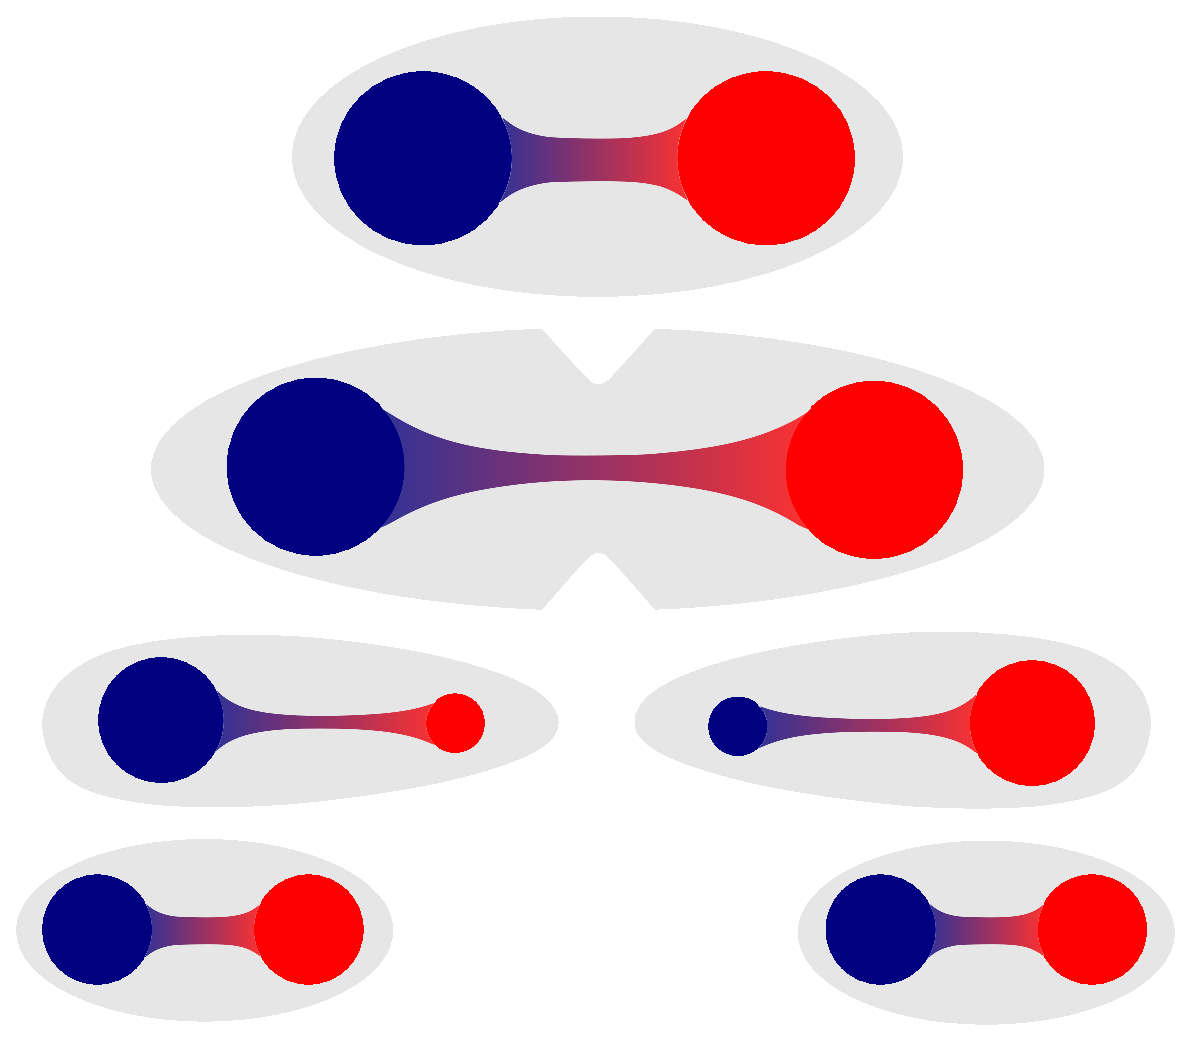
\includegraphics[width=0.7\textwidth]{images/QuarkConfinement.eps}
            }{
                % Size of image in report class
                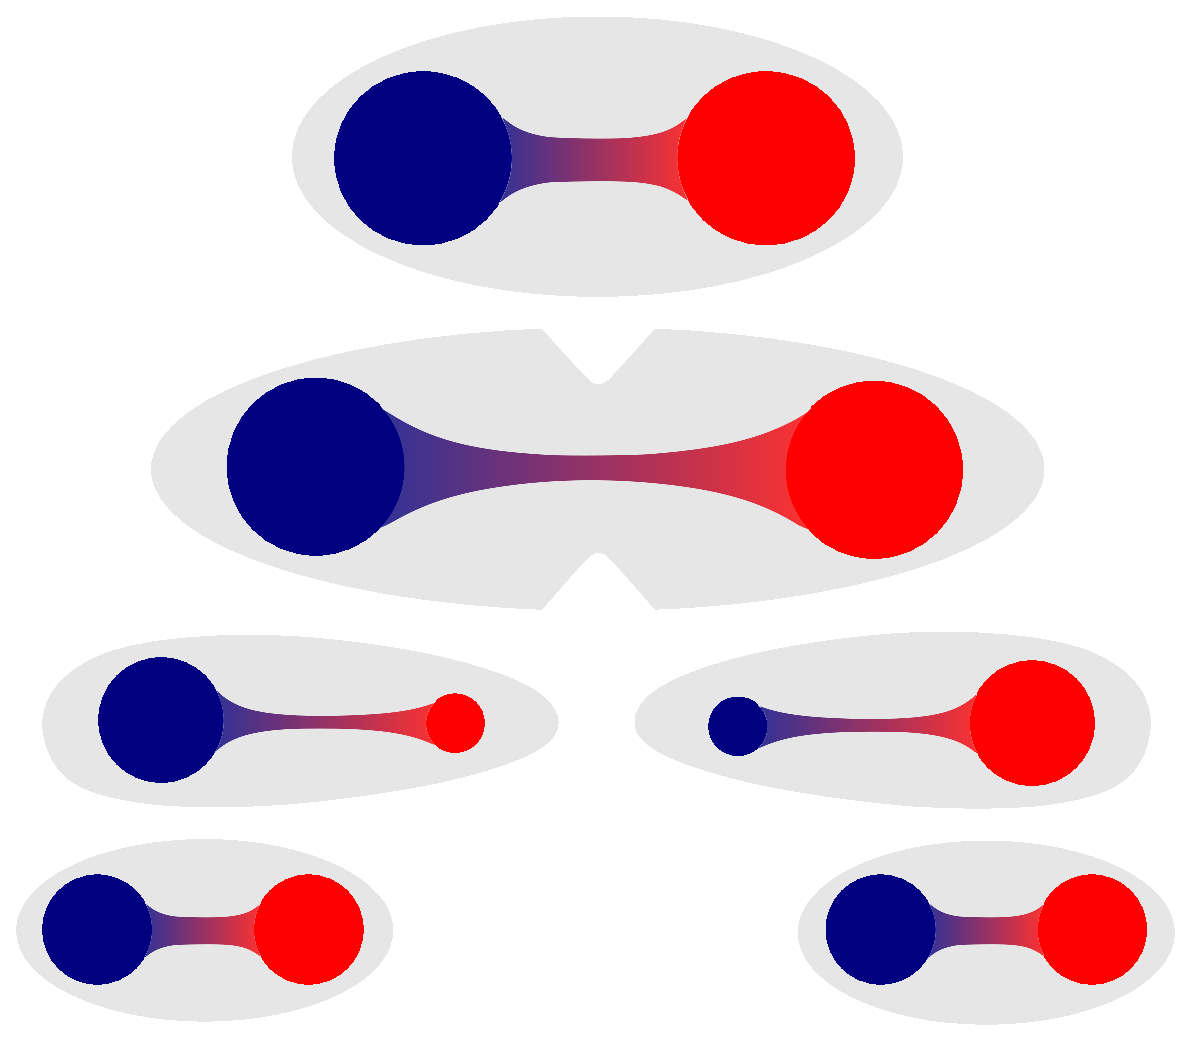
\includegraphics[width=0.7\textwidth]{images/QuarkConfinement.eps}
            }
        };
        % Draw the coordinate system
        \begin{scope}[x={(image.south east)},y={(image.north west)}]
            \draw[thick,|-|] (0.35, 1.03) -- node[above, midway] {\large $r$} (0.65, 1.03);
            \draw[thick,->] (0, 1) -- node[right, midway] {\large time} (0, 0.8);
        \end{scope}
    \end{tikzpicture}
    \caption{As a quark\index{quark} (red) and an antiquark\index{antiquark} (blue) in a meson\index{meson} are pulled away from each other (distance $r$ increases), the energy needed increases until the string tension of the flux tube\index{flux tube} (blue to red gradient) between the particles is sufficient enough, thus the flux tube break, known as string breaking\index{string breaking}, and the energy stored in the flux tube creates a new quark and antiquark such that there is now two mesons. That a quark and an antiquark can never exist on its own is know as colour confinement\index{colour confinement}\index{confinement|see{colour confinement}}. Inspired by Ref. \cite{institutoDeFisicaCorpuscular_numericalApproach_2016}.}
    \label{fig:QuarkConfinement}
\end{figure}

A possible mechanism resulting in the linearly growing potential is that the gluon field of the strong interaction creates a narrow colour \emph{flux tube} (also known as a string) between the quark and antiquark \cite{brandt_effectiveStringDescriptionOfConfiningFluxTubes_2016}. Thus the potential becomes $V(r) \approx \sigma r$ for $r$ being the interquark distance and $\sigma$ being the string tension. At some point the amount of energy in the flux tube becomes sufficient enough and the tube breaks, which is known as \emph{string breaking}\index{string breaking}, see \cref{fig:QuarkConfinement}. As an analogy we consider an elastic band: As it is stretched the energy stored in the band grows and at some point the band snaps. Instead of one elastic band with two end points you are now left with two bands with each two ends. Thus new ends are created due to the release of stored energy. Translating this to a system of a meson, \cref{fig:QuarkConfinement}, it can be seen that at some point it becomes energetically favourable for the string to break and create a quark-antiquark pair (pair-production), and thus resulting in two mesons.

\index{confinement|)}




\section{Lattice Schwinger model exhibiting confinement} \label{sec:LatticeSchwingerModelAndConfienemt}

In \cref{sec:SpinModelOfTheLatticeSchwingerModel} we remodelled the (1+1)-dimensional lattice Schwinger model into containing spin operators, \cref{eq:LatticeSchwingerModelHamiltonianSpin}.
% \begin{align} \label{eq:Confienement_LatticeSchwingerModelHamiltonianSpin}
%     H &= \sum_n \left[ (-1)^{n+1} \frac{m}{2} \sigma_n^z - \frac{1}{2a} \left( \sigma_n^+ S_n^+ \sigma_{n+1}^- + \mathrm{h.c.} \right) + \frac{a^3 q^2 S^2}{2} \left( S_n^z \right)^2 \right] \: .
% \end{align}
For this we have chosen to define the spin states as $\ket{0} = (1,\, 0)^T$ and $\ket{1} = (0,\, 1)^T$, i.e. $\ket{0}$ is the excited state and $\ket{1}$ is the ground state, for the spin-\half system, since this is easy to generalise to larger spin systems as spin-1 by expanding the existing states with a new $0$-row and stating a new state with only a $1$-row at the last row (the $(2S+1)^\mathrm{th}$ row), i.e. for spin-1: $\ket{0} = (1,\, 0,\, 0)^T$, $\ket{1} = (0,\, 1,\, 0)^T$ and $\ket{2} = (0,\, 0,\, 1)^T$. This definition of the states for the spin-\half results in the spin step operators to switch their normal definition such that we have
\begin{align} \label{eq:StepOperatorsSpin1/2}
    \sigma^+ = \begin{pmatrix} 0 & 0 \\ 1 & 0 \end{pmatrix} \: , \quad \text{and} \quad
    \sigma^+ = \begin{pmatrix} 0 & 1 \\ 0 & 0 \end{pmatrix} \: .
\end{align}
The Pauli matrix $\sigma^z$ still remains the usual
\begin{align} \label{eq:PauliZOperatorSpin1/2}
    \sigma^z &= \begin{pmatrix} 1 & 0 \\ 0 & -1 \end{pmatrix} \: .
\end{align}
In \cref{eq:LatticeSchwingerModelHamiltonianSpin} $S^z$ and $S^+$ are the spin-$S$ analogies of the Pauli matrix $\sigma^z$ and the spin step operator $\sigma^+$ respectively. Due to us wanting to simulate confinement, the gauge field spin operators is required to be that of a spin-1 system\footnote{They are required to have integer spin, since this enables us to have a state of zero field. Spin-1 is just the lowest non-trivial integer spin, thus it is easier to work with.}, since the possibility of zero field between the mesons is necessary. The spin operators $S^z$ and $S^+$ of a spin-1 system can be calculated by first coupling the spin projections to the states: \ldots
\begin{align} \label{eq:SpinOperatorsSpin1}
    S^+ &= \begin{pmatrix} 0 & 0 & 0 \\ \sqrt{2} & 0 & 0 \\ 0 & \sqrt{2} & 0 \end{pmatrix}
    \: , \quad \text{and} \quad
    S^z = \begin{pmatrix} 1 & 0 & 0 \\ 0 & 0 & 0 \\ 0 & 0 & -1 \end{pmatrix} \: .
\end{align}

Letting the gauge field be represented by spin-1 operators, thus setting $S = 1$, results in the Hamiltonian
\begin{align} \label{eq:LatticeSchwingerModelHamiltonianSpin_Actual}
    H &= \sum_n \left[ (-1)^{n+1} \frac{m}{2} \sigma_n^z - \frac{1}{2a} \left( \sigma_n^+ S_n^+ \sigma_{n+1}^- + \mathrm{h.c.} \right) + \frac{a^3 q^2}{2} \left( S_n^z \right)^2 \right] \: ,
\end{align}
with the spin operators defined in \cref{eq:StepOperatorsSpin1/2,eq:PauliZOperatorSpin1/2,eq:SpinOperatorsSpin1}.



\subsection{Computing the states} \label{sec:StateComputing}

To be able to simulate confinement it is necessary to know the interpretation of the states, i.e. for matter states the above mentioned definition of $\ket{0}$ and $\ket{1}$ necessitates $\ket{1_n}$ to be interpreted as the presence of a particle if $n$ is even and a vacant site if $n$ is odd, while $\ket{0_n}$ means the site is vacant for even $n$ and that an antiparticle is present for odd $n$.

We add to the generator, \cref{eq:GeneratorU(1)SymmetryDiscretized}, a constant of $q[(-1)^n - 1]/2$ which ensures particles and antiparticles an intuitive charge \cite{panyella_masterThesis_2019},
\begin{align} \label{eq:GeneratorWithExtraConstant}
    G_n = \frac{E_n - E_{n-1}}{a} - q \psi_n\dagger \psi_n - \frac{(-1)^n - 1}{2} \: .
\end{align}
As with the Hamiltonian in \cref{sec:SpinModelOfTheLatticeSchwingerModel} the generator is remodelled using the spin formalism with $S=1$, thus
\begin{align} \label{eq:GeneratorU(1)SymmetrySpinVersion} \index{generator!of U(1) symmetry!discretized!with spin}\index{generator!of U(1) symmetry}
    G_n = q \left( S_n^z - S_{n-1}^z - \frac{1}{2} \big[ - \sigma_n + (-1)^n \big] \right) \: .
\end{align}
%
\begin{table}[t]
    \centering
    \begin{tabular}{|c|c|c|}
        \hline
        State & \multicolumn{2}{c|}{$G_n / q$} \\
         & Even $n$ & Odd $n$ \\ \hline
        $\ket{\, 0_g\, 0_m\, 0_g}$ & $0$ & $1$ \\ \hline
        $\ket{\, 0_g\, 1_m\, 0_g}$ & $-1$ & $0$ \\ \hline
        $\ket{\, 0_g\, 0_m\, 1_g}$ & $1$ & $2$ \\ \hline
        $\ket{\, 0_g\, 1_m\, 1_g}$ & $0$ & $1$ \\ \hline
        $\ket{\, 0_g\, 0_m\, 2_g}$ & $2$ & $3$ \\ \hline
        $\ket{\, 0_g\, 1_m\, 2_g}$ & $1$ & $2$ \\ \hline
        $\ket{\, 1_g\, 0_m\, 0_g}$ & $-1$ & $0$ \\ \hline
        $\ket{\, 1_g\, 1_m\, 0_g}$ & $-2$ & $-1$ \\ \hline
        $\ket{\, 1_g\, 0_m\, 1_g}$ & $0$ & $1$ \\ \hline
        \multicolumn{3}{|c|}{\textsl{continued to the right}} \\ \hline
    \end{tabular}
    \hspace{.3em}
    \begin{tabular}{|c|c|c|}
        \hline
        State & \multicolumn{2}{c|}{$G_n / q$} \\
         & Even $n$ & Odd $n$ \\ \hline
        \multicolumn{3}{|c|}{\textsl{continued from the left}} \\ \hline
        $\ket{\, 1_g\, 1_m\, 1_g}$ & $-1$ & $0$ \\ \hline
        $\ket{\, 1_g\, 0_m\, 2_g}$ & $1$ & $2$ \\ \hline
        $\ket{\, 1_g\, 1_m\, 2_g}$ & $0$ & $1$ \\ \hline
        $\ket{\, 2_g\, 0_m\, 0_g}$ & $-2$ & $-1$ \\ \hline
        $\ket{\, 2_g\, 1_m\, 0_g}$ & $-3$ & $-2$ \\ \hline
        $\ket{\, 2_g\, 0_m\, 1_g}$ & $-1$ & $0$ \\ \hline
        $\ket{\, 2_g\, 1_m\, 1_g}$ & $-2$ & $-1$ \\ \hline
        $\ket{\, 2_g\, 0_m\, 2_g}$ & $0$ & $1$ \\ \hline
        $\ket{\, 2_g\, 1_m\, 2_g}$ & $-1$ & $0$ \\ \hline
    \end{tabular}
    \caption{The eigenvalues of the generator from \cref{eq:GeneratorU(1)SymmetrySpinVersion} for the 18 configurations of two gauge fields (denoted with a $g$) with spin-$1$ and a matter field (denoted with an $m$) with spin-\half between them.}
    \label{tab:EigenvaluesOfGenerator}
\end{table}
%
Calculating now the eigenvalues of the the generator for the 18 different configurations of two spin-1 gauge fields surrounding a spin-\half matter field results in \cref{tab:EigenvaluesOfGenerator}. Examining the table one may notice that for even sites $\ket{\, 0_g\, 1_m\, 1_g}$ and $\ket{\, 0_g\, 0_m\, 1_g}$ ($m$ and $g$ is here denoting matter fields and gauge fields respectively) only differ by the presence of a particle and of the value $q$. The same can be shown for odd sites $\ket{\, 1_g\, 0_m\, 0_g}$ and $\ket{\, 1_g\, 1_m\, 0_g}$, which only differ by the presence of an antiparticle and by the values $-q$. Thus by understanding the eigenvalue of $G_n$ as a static background (anti)particle \cite{panyella_masterThesis_2019}, it is shown that $q$ is in fact, as stated in \cref{sec:ContinuumQFT_LocalU(1)GaugeInvariance}, the charge of a particle and likewise $-q$ the charge of an antiparticle.

Now the direction of the electric field is to be found. For this we postulate $\ket{1_g}$ to be zero field, which is in agreement with $G_n \ket{\, 1_g\, 0_m\, 1_g} = 0 \ket{\, 1_g\, 0_m\, 1_g}$ for even $n$ since this indicates neither a field nor a particle, i.e. vacuum, which is expected to have zero charge. Using now the gauge interaction operator $\sigma_n^+ S_n^+ \sigma_{n+1}^-$ from the Hamiltonian, \cref{eq:LatticeSchwingerModelHamiltonianSpin_Actual}, on the matter site and thus right hand link of $\ket{\, 1_g\, 0_m\, 1_g}$ one gets $\sigma_n^+ S_n^+ \sigma_{n+1}^- \ket{\, 1_g\, 0_m\, 1_g} = \ket{\, 1_g\, 1_m\, 2_g}$, thus we have created a particle and changed the right hand gauge field. We would like the field to point from particles to antiparticles, thus $\ket{2_g}$ must be interpreted as an electric field pointing right. The two observations of $\ket{1_g}$ and $\ket{2_g}$ happens to be consistent with the rest of the states, thus the interpretations become $\ket{0_g} = \ket{\leftarrow}$, $\ket{2_g} = \ket{\rightarrow}$ and $\ket{1_g} = \ket{0}$, the latter indicating zero field.



\subsection{Confinement and string breaking} \label{sec:ConfienementAndStringBreakingAnalyticalAndNumerical}

\subsubsection{Analytical study: Variables favourable for string breaking}

\begin{figure}[t]
    \centering
    \begin{tikzpicture}[
        % Definition of node styles
        particle/.style={circle, fill=red!100, very thick, minimum size=2mm},
        antiparticle/.style={circle, fill=blue!100, very thick, minimum size=2mm},
        emptysite/.style={circle, draw=black!0, minimum size=2mm},
        node distance = 2.5cm,
        ]
        % Nodes
        \node[antiparticle]     (firstParticle) {};
        \node[emptysite]        (firstAntiparticle)     [right=of firstParticle] {};
        \node[emptysite]        (secondParticle)        [right=1.25cm of firstAntiparticle] {};
        \node[particle]         (secondAntiparticle)    [right=of secondParticle] {};
        % Links
        \draw[dashed, middlearrow={stealth reversed}] (firstParticle.east) -- (secondAntiparticle.west);
        % Name of the system
        % \node at (0,1.75) {\large \underline{System A}};
        \node at (-1.75,.9) {\large \underline{System A:}};
        % Distances
        \draw[thick,|-|] (0, 0.65) -- node[above, midway] {\large $R=la$} (7.6, 0.65);
    \end{tikzpicture}
    \\
    \vspace{2em}
    \begin{tikzpicture}[
        % Definition of node styles
        particle/.style={circle, fill=red!100, very thick, minimum size=2mm},
        antiparticle/.style={circle, fill=blue!100, very thick, minimum size=2mm},
        node distance = 2.5cm,
        ]
        % Nodes
        \node[antiparticle]     (firstParticle) {};
        \node[particle]         (firstAntiparticle)     [right=of firstParticle] {};
        \node[antiparticle]     (secondParticle)        [right=1.25cm of firstAntiparticle] {};
        \node[particle]         (secondAntiparticle)    [right=of secondParticle] {};
        % Links
        \draw[dashed, almostmiddlearrow={stealth reversed}] (firstParticle.east) -- (firstAntiparticle.west);
        \draw[dashed, almostmiddlearrow={stealth reversed}] (secondParticle.east) -- (secondAntiparticle.west);
        % Name of the system
        % \node at (0,1.85) {\large \underline{System B}};
        \node at (-1.75,.9) {\large \underline{System B:}};
        % Distances
        \draw[thick,|-|] (0, 0.65) -- node[above, midway] {\large $(R-a)/2$} (2.95, 0.65);
        \draw[thick,|-|] (2.95, 0.65) -- node[above, midway] {\large $a$} (4.65, 0.65);
        \draw[thick,|-|] (4.65, 0.65) -- node[above, midway] {\large $(R-a)/2$} (7.6, 0.65);
    \end{tikzpicture}
    \caption{The two states for which the study of analytical string breaking is performed. The energy of the two systems is calculated and it is found, that for $R < R_0$ the energy of System A, a meson with interquark distance $R=la$, is smallest, but at the string breaking length $R_0$ this changes, and it is energy efficient to break the flux tube and create a new quark-antiquark pair, such that there is now two mesons with interquark distance $(R-a)/2$ each.}
    \label{fig:SystemForAnalyticalSimulationOfConfinementAndStringBreaking}
\end{figure}

For the analytical study of confinement and string breaking the systems shown in \cref{fig:SystemForAnalyticalSimulationOfConfinementAndStringBreaking} are used. System A illustrates a meson with interquark distance $R = la$ for which $a$ is the lattice spacing and $l$ is an odd integer fulfilling $(l-1)/2$ also being an odd integer. When $R$ becomes sufficient enough, $R_0$, string breaking occurs, thus we will now be in system B instead, where there is now two mesons with interquark distance $(R-a)/2$ each. In this section the connection between the values of lattice spacing, mass and charge favourable for string breaking will be found by computing and comparing the energy of the two systems.

The energy of the systems is found by computing the expectation value of the Hamiltonian \cref{eq:LatticeSchwingerModelHamiltonianSpin_Actual} with respect to the two states respectively. Let us consider the three terms of the Hamiltonian, for convenience defined $H = \sum_n \left[ H_m + H_I + H_E \right]$, individually. Firstly we will consider the interaction term $H_I$, which consists of step operators and their Hermitian conjugates. It is known that $\mel**{s'}{\sigma^\pm}{s} \propto \delta_{s',s+1}$ for states $\ket{s}$ and $\ket{s'}$, and equally for $S^\pm$, thus $\expval{H_I} = \expval{H_I}{\Psi} = 0$ for $\ket{\Psi}$ being the state of either System A or B.
Now let us consider the mass term $H_m$, by considering the expectation value with a (anti)quark present and at a vacant site. Remember that $\sigma^z\ket{0_m} = 1$ and $\sigma^z\ket{1_m} = -1$, thus for even $n$ we have
\begin{align}
\begin{split}
    \expval{H_m}_{1_m} &= \mel**{1_m}{(-1)^{n+1} \frac{m}{2} \sigma_n^z}{1_m}
        = \mel**{1_m}{-1 \frac{m}{2} (-1)}{1_m}
        = \frac{m}{2} \: ,
    \quad \text{and} \\
    \expval{H_m}_{0_m} &= \mel**{0_m}{(-1)^{n+1} \frac{m}{2} \sigma_n^z}{0_m}
        = \mel**{0_m}{-1 \frac{m}{2} 1}{0_m}
        = -\frac{m}{2} \: ,
\end{split}
\end{align}
thus by inserting a quark the energy has increased with $\expval{H_m}_{1_m} - \expval{H_m}_{0_m} = m$. The same can be shown for the antiquark where $(-1)^{n+1}$ changes the sign such that the energy from the presence of an antiquark results in the energy increase $\expval{H_m}_{0_m} - \expval{H_m}_{1_m} = m$ (for odd $n$). Thus the energy from the mass term is $E_m = km$ for $k$ being the number of quarks and antiquarks in the system.
Lastly we are considering the electric field term $H_E$. For this term it is trivial to observe that $(S^z)^2\ket{0_g} = 1\ket{0_g}$, $(S^z)^2\ket{1_g} = 0 \ket{1_g}$ and $(S^z)^2\ket{2_g} = 1\ket{2_g}$, thus for every link $l$ with a non-zero field the energy is $a^3 q^2 / 2$.

From the above observations the expectation value of the Hamiltonian becomes\footnote{Actually the expectation value of the Hamiltonian lacks a constant offset, but since we will be comparing the energy of two systems the offset would disappear anyways, thus it have been omitted in \cref{eq:ExpectationValueOfHamiltonian}.}
\begin{align} \label{eq:ExpectationValueOfHamiltonian}
    \expval{H} &= km + \frac{a^3 q^2}{2}l
\end{align}
with $k$ being the number of quarks and antiquarks and $l$ satisfying $L=la$ as before. Using \cref{eq:ExpectationValueOfHamiltonian} the energy of the two systems in \cref{fig:SystemForAnalyticalSimulationOfConfinementAndStringBreaking} becomes
\begin{align}
    E_A &= 2m + \frac{a^3 q^2}{2}l \: ,
    \quad \text{and} \quad
    E_B = 4m + \frac{a^3 q^2}{2}(l-1) \: .
\end{align}
Equating the two energies yields the following relation between the properties of the system,
\begin{align} \label{eq:StringBreakingFavourableValues}
    a = \sqrt[3\:\:\,]{\frac{4m}{q^2}} \: ,
\end{align}
for which string breaking is energetically favourable.



\subsubsection{Numerical study: Confinement and string breaking}

\begin{figure}[t]
    \centering
    \begin{tikzpicture}[
        % Definition of node styles
        particle/.style={circle, fill=red!100, very thick, minimum size=2mm},
        antiparticle/.style={circle, fill=blue!100, very thick, minimum size=2mm},
        emptysite/.style={circle, draw=black!40, minimum size=2mm},
        node distance = 1.75cm,
        ]
        % Nodes
        \node[label={[label distance=.1cm]above:{\large $E_n$ direction}}, label={[label distance=.1cm]below:{\large Site number}}] (text) {\large Configuration};
        \node[antiparticle, label={[label distance=.3cm]below:{\large $1$}}] (firstParticle) [right=.5cm of text] {};
        \node[emptysite, label={[label distance=.3cm]below:{\large $2$}}] (firstAntiparticle) [right=of firstParticle] {};
        \node[emptysite, label={[label distance=.3cm]below:{\large $3$}}] (secondParticle) [right=of firstAntiparticle] {};
        \node[particle, label={[label distance=.3cm]below:{\large $4$}}] (secondAntiparticle) [right=of secondParticle] {};
        % Links
        \draw[dashed] (firstParticle.east) -- node[above=0.55cm, midway, black] {\Large $\leftarrow$} (firstAntiparticle.center);
        \draw[dashed] (firstAntiparticle.center) -- node[above=0.55cm, midway, black] {\Large $\leftarrow$} (secondParticle.center);
        \draw[dashed] (secondParticle.center) -- node[above=0.55cm, midway, black] {\Large $\leftarrow$} (secondAntiparticle.west);
        % Name of the state
        \node at (-1,1.5) {\large \underline{State $\varphi$}};
    \end{tikzpicture}
    \newline
    \vspace{.1em}
    \begin{tikzpicture}[
        % Definition of node styles
        particle/.style={circle, fill=red!100, very thick, minimum size=2mm},
        antiparticle/.style={circle, fill=blue!100, very thick, minimum size=2mm},
        node distance = 1.75cm,
        ]
        % Nodes
        \node[label={[label distance=.1cm]above:{\large $E_n$ direction}}, label={[label distance=.1cm]below:{\large Site number}}] (text) {\large Configuration};
        \node[antiparticle, label={[label distance=.3cm]below:{\large $1$}}] (firstParticle) [right=.5cm of text] {};
        \node[particle, label={[label distance=.3cm]below:{\large $2$}}] (firstAntiparticle) [right=of firstParticle] {};
        \node[antiparticle, label={[label distance=.3cm]below:{\large $3$}}] (secondParticle) [right=of firstAntiparticle] {};
        \node[particle, label={[label distance=.3cm]below:{\large $4$}}] (secondAntiparticle) [right=of secondParticle] {};
        % Links
        \draw[dashed] (firstParticle.east) -- node[above=0.55cm, midway, black] {\Large $\leftarrow$} (firstAntiparticle.west);
        \draw[dashed, black!40] (firstAntiparticle.east) -- node[above=0.55cm, midway, black] {\Large $0$} (secondParticle.west);
        \draw[dashed] (secondParticle.east) -- node[above=0.55cm, midway, black] {\Large $\leftarrow$} (secondAntiparticle.west);
        % Name of the state
        \node at (-1,1.5) {\large \underline{State $\chi$}};
    \end{tikzpicture}
    \caption{The two states for which the numerical study of string breaking is performed. The system starts in state $\varphi$ with the variables set to be favourable for string breaking, thus the system will over time go to state $\chi$. The red and blue circles are quarks and antiquarks respectively, the grey outlined circles are sites with neither a quark nor an antiquark, and the dashed lines is the gauge field (electric field). The direction of the electric field between the quarks and antiquarks is noted above the lattice links, and the grey dashed line reflects the electric field not being present.}
    \label{fig:SystemForNumericalSimulationOfConfinementAndStringBreaking}
\end{figure}

For the numerical study of confinement and string breaking the system will consist of the two states shown in \cref{fig:SystemForNumericalSimulationOfConfinementAndStringBreaking}. These are actually the same as for the analytical study, \cref{fig:SystemForAnalyticalSimulationOfConfinementAndStringBreaking}, with $l=3$, thus we work with three links and four matter sites ($N=4$). Instead of examining the energy of the two systems we will here examine the \emph{fidelity} of the two states with the time evolving initial state, $\varphi(t)$. Starting from the definition of the fidelity\index{fidelity} of two states $\ket{\Phi}$ and $\ket{\Psi}$, the norm square of the inner product of the two states, it can be shown that this equals the expectation value with respect to one of the states of the \emph{density operator}\footnote{The density operator contains all the physically significant information that is obtainable for an ensemble \cite{sakurai_modernQM_2017}.}\index{density operator} of the other state,
\begin{align}
    \abs{\innerproduct{\Phi}{\Psi}}^2
    = \innerproduct{\Phi}{\Psi}\innerproduct{\Psi}{\Phi}
    = \mel**{\Phi}{\big( \outerproduct{\Psi} \big)}{\Phi} \: .
\end{align}
Thus for the numerical study we will be using the \textsc{Python} module \textsc{QuTiP}\footnote{For this the \textsc{QuTiP} version 4.5.0 is used.} and its master equation solver \textsf{mesolve}, which time evolves its input state relative to the constructed Hamiltonian, \cref{eq:LatticeSchwingerModelHamiltonianSpin_Actual}, and give as output the expectation value of this time evolved state and the density operators of $\ket{\varphi}$ and $\ket{\chi}$ provided the solver. \cref{fig:stringBreakingNumerical} is the resulting graph of the fidelity, for the string breaking favourable values $m=1$, $q=1$ and $a = \sqrt[3\:\:]{4m/q^2} \approx \num{1.59}$ (found in \cref{eq:StringBreakingFavourableValues}), and the two states
\begin{align}
    \varphi &= \ket{\, 1_m\, 0_g\, 1_m\, 0_g\, 0_m\, 0_g\, 0_m} \: \quad \text{and} \quad \chi = \ket{\, 1_m\, 0_g\, 0_m\, 1_g\, 1_m\, 0_g\, 0_m} \: .
\end{align}

\begin{figure}[t]
    \centering
    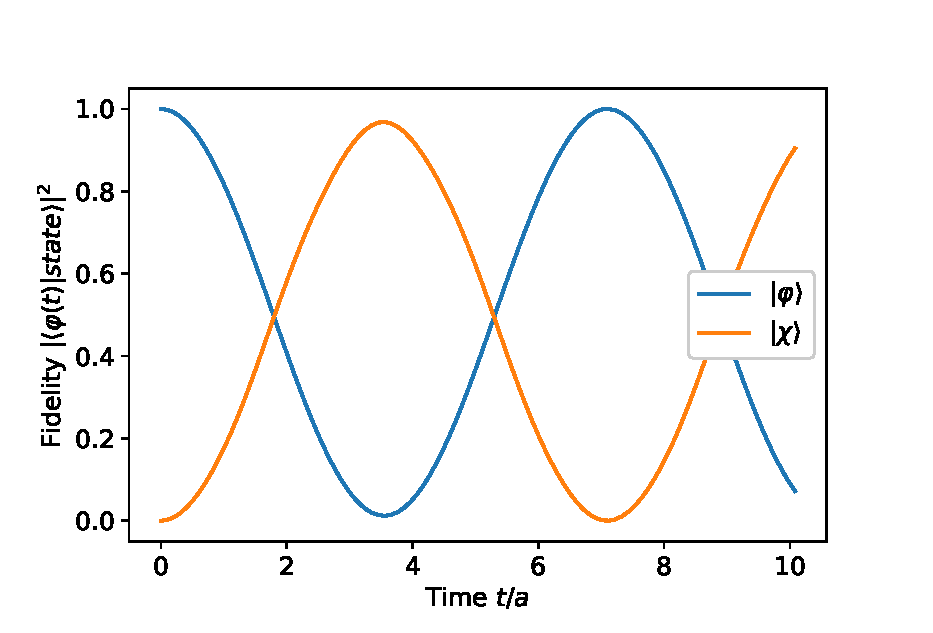
\includegraphics[width=\textwidth]{text/images/stringBreakingNumerical.eps}
    \caption{The fidelity of the time evolved initial state, $\ket{\varphi(t)}$ for the system and the initial state, $\ket{\varphi}$, and the state expected after string breaking, $\ket{\chi}$. Here the string breaking favourable values $m=1$, $q=1$ and $a = \sqrt[3\:\:]{4m/q^2} \approx \num{1.59}$ (found in \cref{eq:StringBreakingFavourableValues}) is used.}
    \label{fig:stringBreakingNumerical}
\end{figure}

As seen at \cref{fig:stringBreakingNumerical} the system starts in state $\ket{\psi}$, i.e. the fidelity $\abs{\innerproduct{\varphi(t=0)}{\varphi}}^2 = 1$, and then proceeds to be almost fully in state $\ket{\chi}$ at $t=\num{3.5}$, i.e. $\abs{\innerproduct{\varphi(t=0)}{\chi}}^2 \approx 1$, as was expected of the system. Now we would expect the system to stay in the new state -- the energy of the new state should be less than that of the initial according to the theory -- but looking at the graph this is not the case. Instead the fidelity looks like a periodic function, thus the system periodically over time changes from state $\ket{\varphi}$ to state $\ket{\chi}$ and back. This is due to \ldots
\ldots Explain the graph \ldots

% Tilstandene oscillerer, fordi dit system er så småt, mere eller mindre. Det er et eksempel på quantum revival (https://en.wikipedia.org/wiki/Quantum_revival), som sker i alle systemer, men er mest prominent i små systemer. Der er ikke særlig mange tilstande, som din begyndelsestilstand er koblet til, så når dens population flyder ud i dem, vil den population komme delvist tilbage igen på et tidspunkt. Og fordi der så ikke er så mange tilstande, kommer den ret hurtigt tilbage, men til gengæld er der ikke perfekt revival, fordi tilstandenes energier ikke er heltalsprodukter af hinanden.




\section{Outlook} \label{sec:Outlook}

In this chapter the string breaking distance $R_0$ was introduced but neither the analytical nor the numerical study reveals its value. I therefore propose this as a further study of the confinement and string breaking using the (1+1)-dimensional lattice Schwinger model. The string breaking distance can then be compared to other studies using the Schwinger model \cite{buyens_confinementAndStringBreaking_2016} and that of numerical quantum chromodynamic models \cite{petkovic_stringBreakingAndQuarkConfinement_2018, bulava_stringBreakingByLightAndStrangeQuarksInQCD_2019}, which states the string breaking distance to be in the range $R_0 \in [15,\, 20]a$ with $a$ still denoting the lattice spacing.

Another interesting further development of this chapter would be to examine the system of the numerical study but with a higher number of lattice sites, thus hoping to show string breaking without the quantum revival effect. Even though increasing the number of lattice sites might result in a more precise results it has a negative effect on the computability of the system, due to its higher complexity thus the functions become more time consuming to compute. The calculations of confinement use a lattice of $N$ sites, with two spins states, and thus $N-1$ links, with three spin states, resulting in the dimension of the problem being $2^N \cdot 3^{N-1}$, i.e. the dimension of the problem increases exponentially. For the case of the numerical study above a lattice with $N=4$ lattice sites have been used, thus the dimensions became $432$, which was computable on a regular laptop. Considering instead $N=20$ lattice sites would yield a problem dimension of $\num{1.2e15}$, which can be difficult for a computer to handle.




\end{document}